\chapter{Evaluationen}
\label{ch:05_evaluation}

% Allgemeine Einleitung.
Nach der Definition der softwaretechnischen Realisierung und dem Aufzeigen erster Grenzen und Eigenheiten der
untersuchten Rendering-Paradigmen in Kapitel 4 werden die implementierten Architekturen isolierten Stresstests
unterzogen.
Das primäre Ziel dieses Kapitels liegt in der objektiven Quantifizierung der zuvor theoretisch beschriebenen
Performance-Engpässe unter einer systematischen Skalierung von Szenenkomplexität und Stil-Entropie.
Um die übergeordneten Forschungsfragen belastbar zu beantworten, definiert der erste Abschnitt zunächst die methodischen
Rahmenbedingungen und technischen Spezifikationen des Versuchsaufbaus.
Darauf aufbauend erfolgt die schrittweise Datenauswertung anhand spezifischer Kontrollgruppen und der gezielten
Untersuchung vermuteter Performance-Engpässe, bevor ein abschließender Macro-Benchmark die gewonnenen Erkenntnisse
ganzheitlich evaluiert.


\section{Evaluationsmethodik \& Experimenten-Design}
\label{sec:0501_evaluation_methodology}

% 5.1 Einleitung.
Das in Kapitel 4 konzipierte Test-Framework fungiert im Folgenden als Messwerkzeug für die empirische Analyse der darin
implementierten Rendering-Pipelines.
Für die objektive und isolierte Betrachtung der verschiedenen postulierten Performance-Engpässe definiert der
vorliegende Abschnitt die methodischen Grundlagen.
Dies umfasst die Formulierung der Hypothesen selbst, die exakte Spezifikation des Test-Systems und des
Variablen-Mappings sowie die Orchestrierung des Versuchsablaufs.

\subsection{{Zielsetzung und Hypothesen der Untersuchung}}
\label{subsec:050101_evaluation_tagets_and_hypothesis}

% Evaluationsziel
Wie in Kapitel 3 dargelegt, weisen die theoretischen Architekturparadigmen des naiven Forward-, Deferred-Uber- und
Deferred-Volume-Renderings spezifische Leistungsmerkmale auf.
Das primäre Ziel der nachfolgenden Testreihen besteht in der isolierten Quantifizierung dieser technologischen
Trade-offs.
Es sollen die individuellen Kipppunkte auf Hardware-Ebene lokalisiert und evaluiert werden.
Dadurch soll vermieden werden eine Pipeline den anderen gegenüber, als inhärent überlegen zu präsentieren.

% Technische Hypothesen.
Auf Basis der in Kapitel 3 dargelegten theoretischen Faktenlage werden für die implementierten Rendering-Pipelines
spezifische Leistungshypothesen formuliert.
Diese Annahmen gilt es im Folgenden durch gezielte Evaluationen objektiv zu verifizieren oder zu falsifizieren.
Die empirische Untersuchung beleuchtet dabei gleichzeitig die hardwaretechnischen Grenzen und strukturellen Schwächen
des verwendeten Evaluations-Frameworks \textit{HyDra}.

% Hypothese Forward.
Für die als Referenz gewählte, naive Forward-Rendering-Pipeline werden zwei primäre Leistungsengpässe postuliert.
Auf GPU-Ebene wird bei steigender Szenen- und Beleuchtungskomplexität erwartet, dass die Kombination aus geometrischem
Fragment-Overdraw und der multiplikativen algorithmischen Komplexität der direkten Beleuchtungsberechnung von
$O(\text{Fragmente} \cdot \text{Lichter})$ zu signifikanten Leistungseinbußen führt (\textbf{Hypothese H1.1}).
Hinsichtlich der CPU-Auslastung wird angenommen, dass das CPU-seitige Filtern und Zuordnen von Lichtquellen pro Objekt
sowie das hochfrequente Binden objektspezifischer Licht-Uniforms einen signifikanten API-Overhead provoziert, welcher
die CPU-Zuweisungszeit bei anwachsender Instanzenanzahl nicht-linear skalieren lässt (\textbf{Hypothese H1.2}).

% Hypothese Deferred_Uber.
Für die klassische Deferred-Pipeline mit einfachem Beleuchtungs-Pass monolithischem Uber-Shader wird postuliert, dass
der signifikanteste Leistungsengpass bei einer hohen räumlichen Stil-Entropie auftritt (\textbf{Hypothese H2}).
Wie in den vorangegangenen Kapiteln theoretisch hergeleitet, erzwingen feingranular gestreute NPR-Effekte divergente
Code-Zweige.
Dies führt auf GPU-Ebene unweigerlich zu ineffizienter \textit{Warp-Divergence} (siehe
\ref{sec:0302_industry_state}).
Begleitet wird dieses Phänomen von einem anwachsenden Registerdruck (\textit{Register Pressure}) bei erhöhter
Stil-Vielfalt.
Diese kombinierten Hardware-Flaschenhälse zwingen die Architektur zu einer sequenziellen Abarbeitung der Pixel und
lassen eine messbare Degradation der Shading-Performance bei stark vermischten Effekten erwarten.

% Hypothese Deferred_Volumes.
Für die Deferred-Pipeline auf Basis von Light-Volumes postuliert \textbf{Hypothese H3}, dass diese Architektur eine hohe
Resilienz gegenüber räumlicher Stil-Entropie aufweist und die Branching-Problematik des Uber-Shaders umgeht.
Der primäre Leistungsengpass dieser Methode wird stattdessen in der Sättigung der Speicherbandbreite vermutet.
Das additive HDR-Blending bei einer hohen Anzahl überlappender Light-Volumes provoziert überproportional viele
Read-Modify-Write- (RMW) Zyklen im Framebuffer (VRAM).
Der Uber-Shader umgeht diesen spezifische Speicher-Bottleneck konstruktionsbedingt.

% Abgrenzung sonstiger Limits.
Im vorliegenden Kapitel werden die untersuchten Limitierungen ausschließlich auf Performance-Ebene betrachtet.
Spezifische harte Implementierungsgrenzen der Pipelines (wie etwa die Uniform-Buffer-Limitierungen der Forward- und
Deferred-Uber-Architekturen) sowie etwaige künstlerische Qualitätsengpässe fließen nicht in die Messreihen ein.
Diese Aspekte wurden bereits in Kapitel~\ref{sec:0403_pipeline_implementations} verortet und evaluiert.

\subsection{{Systemkonfiguration und Variablen-Mapping}}
\label{subsec:050102_evaluation_configuration_and_variable_mapping}

% Einleitung
Im Folgenden werden die Referenzdaten der Testumgebung und des verwendeten Software-Stacks beschreiben.
Weiterhin werden die für die testreihen angewendeten unabhängigen Variablen, abhängigen Variablen (Metriken) sowie die
entsprechenden Kontrollvariablen dargelegt udn definiert.

% Einleitung zur Systemkonfiguration.
Die in Tabelle~\ref{tab:hardware_specs} aufgezeigten Hardware-Spezifikationen bestimmen die absoluten physikalischen
Leistungsgrenzen des Systems.
Die in Tabelle~\ref{tab:software_specs} dokumentierten Software-Schnittstellen und Treiber-Versionen definieren die
CPU-seitige Code-Optimierung sowie den grundlegenden API-Overhead.

% Hardware-Tabelle
\begin{table}[h]
    \centering
    \caption{Spezifikation der primären Test-Hardware.}
    \label{tab:hardware_specs}
    \renewcommand{\arraystretch}{1.2}
    \begin{tabularx}{\textwidth}{@{} l X @{}}  % <-- Geändert auf tabularx und \textwidth
        \toprule
        \textbf{Hardware-Komponente}      & \textbf{Spezifikation / Wert}                      \\
        \midrule
        Prozessor (CPU)                   & Intel Core i5-6600K @ 4\times~3.50\,GHz           \\
        Hauptspeicher (RAM)               & 16\,GB DDR4 (Dual-Channel) @ 3000\,MT/s            \\
        Grafikkarte (GPU)                 & NVIDIA GeForce GTX 1660                            \\
        GPU-Architektur                   & Turing (TU116)                                     \\
        VRAM-Kapazität                    & 6\,GB GDDR5                                        \\
        Theoretische VRAM-Bandbreite      & 192,1\,GB/s                                        \\
        Raster Operation Pipelines (ROPs) & 48                                                 \\
        \bottomrule
    \end{tabularx}
\end{table}

% Software-Tabelle
\begin{table}[h]
    \centering
    \caption{Spezifikation der Software-Umgebung und API-Schnittstellen.}
    \label{tab:software_specs}
    \renewcommand{\arraystretch}{1.2}
    \begin{tabularx}{\textwidth}{@{} l X @{}}  % <-- Geändert auf tabularx und \textwidth
        \toprule
        \textbf{Software / API} & \textbf{Version}               \\
        \midrule
        Betriebssystem          & Linux Mint 22.3 (Kernel 6.8.0) \\
        Grafiktreiber           & NVIDIA 595.71.05               \\
        C++ Compiler            & GCC 13.3.0                     \\
        Anwendungs-Framework    & raylib 5.5                     \\
        Grafik-API              & OpenGL 3.3.0 Core Profile      \\
        Shading Language        & GLSL 3.30                      \\
        \bottomrule
    \end{tabularx}
\end{table}

% Einleitung unabhängige Variablen.
Nach der Definition der Hardware- und Software-Spezifikationen erfordert das Evaluation-Design eine exakte Abgrenzung
der unabhängigen Variablen.
Diese Parameter manipuliert das Framework während der Testreihen systematisch.
Es sollen Leistungsgrenzen der Hardware isoliert provoziert werden.
Tabelle~\ref{tab:independent_vars} fasst das Variablen-Mapping zusammen.

% Tabelle der unabhängigen Variablen
\begin{table}[htbp]
    \centering
    \caption{Spezifikation der unabhängigen Variablen und deren Zuordnung zu den Test-Suits.}
    \label{tab:independent_vars}
    \small
    \renewcommand{\arraystretch}{1.1}
    \begin{tabularx}{\textwidth}{@{} l l l >{\raggedright\arraybackslash}X @{}}
        \toprule
        \textbf{Parameter}           & \textbf{Wertebereich} & \textbf{Test-Suite} & \textbf{Beschreibung \& Zweck}                                                                                            \\
        \midrule
        \texttt{activeRenderPath}    & \textit{Enum}         & Alle Suiten         & Die primäre architektonische
        Variable.
        Rotiert durch Forward, Deferred-Uber und Deferred-Volume.\\
        \texttt{currentLodIndex}     & 0 bis 4               & 5.2.1               & Skaliert den geometrischen
        Detailgrad pro Objekt.\\
        \texttt{activeObstacleCount} & bis 50.000            & 5.2.2, 5.2.3, 5.2.3 & Anzahl der gerenderten Instanzen.
        Forciert CPU-Overhead oder Z-Achsen-Overdraw-Dichte.\\
        \texttt{renderResolution}    & 480p bis 4K           & 5.3.1               & Absolute Render-Auflösung zur
        Messung der Fill-Rate. \\
        \texttt{renderFloor}         & \textit{Boolean}      & 5.3.2               & Erzeugt eine Basis-Bandbreitenlast
        (Max Fill-Rate) durch eine raumfüllende Geometrie.\\
        \texttt{activeLightCount}    & 10 bis 5.000          & 5.4.1, 5.4.2.2      & Anzahl der aktiven dynamischen
        Lichter im Frustum.\\
        \texttt{lightIntensity}      & 0,5 bis 20,0          & 5.4.2.1             & Multiplikator für den Lichtradius.
        Forciert RMW-Speicher-Sättigung.\\
        \texttt{useClusteredStyles}  & \textit{Boolean}      & 5.5.1               & Steuert die stilistische Entropie.
        Schaltet zwischen sortierter und gestreuter Verteilung von Effekten um.\\
        \texttt{enableGooch/Toon}    & 1 bis 3 Stile         & 5.5.2               & Stil-Kombinatorik.
        Skaliert die Anzahl der gleichzeitig in einem Frame evaluierten Shading-Modelle.\\
        \texttt{kuwaharaRadius}      & 2 bis 16              & 5.5.3               & Filtergröße für den
        Kuwahara-Kernel.
        Dient der Sättigung der Textur-Bandbreite.\\
        Feature Accumulation         & Pass 1 bis 4          & 5.6               & Kumulative Aktivierung von Geometrie, Basis-Shading und hoher Stil-Entropie über einen determinierten Kamerapfad. \\
        \bottomrule
    \end{tabularx}
\end{table}

% Einleitung abhängigen Variablen
Im direkten Gegenzug zu den manipulierten Parametern erfasst das Telemetrie-Modul des Frameworks eine Reihe
quantitativer Messgrößen.
Diese abhängigen Variablen bilden die empirische Datengrundlage der Evaluationen.
Um die Leistung der Hardware- und Software-Ebenen isoliert beurteilen zu können, werden die Daten pro Frame aggregiert
und zur späteren statistischen Auswertung in das tabellarisch aufgearbeitet.
Tabelle~\ref{tab:dependent_vars} beschreibt die extrahierten Leistungs- und Szenenmetriken.
Die GPU-Laufzeiten werden dabei über asynchrone Hardware-Queries ermittelt, um ein Blockieren der CPU-Pipeline zu
verhindern.

% Tabelle der abhängigen Variablen
\begin{table}[htbp]
    \centering
    \caption{Spezifikation der abhängigen Variablen (Aufzeichnungsmetriken des Telemetrie-Moduls).}
    \label{tab:dependent_vars}
    \small
    \renewcommand{\arraystretch}{1.2}
    \begin{tabularx}{\textwidth}{@{} l l >{\raggedright\arraybackslash}X @{}}
        \toprule
        \textbf{Metrik}           & \textbf{Kategorie} & \textbf{Beschreibung}                                                                                   \\
        \midrule
        \texttt{cpuLogicMs}       & CPU / Host         & Dauer des Logik-Passes (Frustum Culling, Sichtbarkeitsprüfung
        und Matrix-Berechnungen).\\
        \texttt{cpuRenderMs}      & CPU / Host         & Dauer der API-Befehlsübermittlung an die Grafikkarte (Draw Call
        Submission).\\
        \texttt{geomMs}           & GPU / Device       & Dauer des asynchronen Hardware-Queries für den Geometrie-Pass
        (Füllen des G-Buffers).
        Wird für Forward Pipeline nicht befüllt.\\
        \texttt{lightMs}          & GPU / Device       & Dauer des asynchronen Hardware-Queries für die Beleuchtung und
        den NPR-Effekte.
        Forward schreibt hier die kombinierte Last aus Geometrie und Beleuchtung, da Geometrie nicht isoliert werden
        kann.\\
        \texttt{totalGpuMs}       & GPU / Device       & Gesamte GPU-Ausführungszeit des Frames.                                                                 \\
        \texttt{totalFrameTimeMs} & System             & Absolute Frame-Time (Delta Time), gemessen über System-Timer
        (\texttt{std::chrono}).\\
        \texttt{activeInstances}  & Szene              & Anzahl der tatsächlich sichtbaren und verarbeiteten
        Objekt-Instanzen nach dem Frustum Culling.\\
        \texttt{activeTris}       & Szene              & Berechnete Summe der gerenderten Dreiecke (Sichtbare Instanzen
        $\times$ Dreiecke pro Mesh-LOD).\\
        \texttt{currentOverdraw}  & Szene              & Theoretischer Overdraw-Faktor, basierend auf der Frustum-Tiefe
        und der räumlichen Instanzdichte.\\
        \bottomrule
    \end{tabularx}
\end{table}

% Einleitung Kontrollvariablen
Den Abschluss des Variablen-Mappings bilden die Kontrollvariablen.
Diese Parameter definieren die statische Baseline des Frameworks.
Um reproduzierbare Ausgangslagen für alle Messreihen zu garantieren, sind diese Werte eingefroren, sofern die jeweilige
Test-Suite sie nicht explizit als unabhängige Variable überschreibt.
Tabelle~\ref{tab:controlled_vars} fasst die Standardkonfiguration der zusammen.
Besonders kritisch für die Validität der Messungen ist die definierte Warm-up-Phase in Echtzeit.

% Tabelle der Kontrollvariablen
\begin{table}[htbp]
    \centering
    \caption{Spezifikation der Kontrollvariablen und der statischen System-Baseline.}
    \label{tab:controlled_vars}
    \small
    \renewcommand{\arraystretch}{1.2}
    \begin{tabularx}{\textwidth}{@{} l l >{\raggedright\arraybackslash}X @{}}
        \toprule
        \textbf{Kategorie}      & \textbf{Kontrollvariable}          & \textbf{Standardwert (Baseline)}                        \\
        \midrule
        Rendering \& Pipeline   & \texttt{use16BitHDR}               & \texttt{true}                                           \\
        & \texttt{renderResolution}          & $1920 \times 1080$ (1080p)\\
        & \texttt{renderFloor}               & \texttt{true}\\
        \midrule
        Verteilung \& Geometrie & \texttt{activeObstacleCount}       & 5.000                                                   \\
        & \texttt{objectSphereRadius}        & 200,0\\
        & \texttt{currentLodIndex}           & 1\\
        & \texttt{useClusteredStyles}        & \texttt{false}\\
        \midrule
        Licht-Physik            & \texttt{ambientLightStrength}      & 1,0\\
        & \texttt{lightIntensity}            & 2,0\\
        & \texttt{useLightSingularity}       & \texttt{false}\\
        \midrule
        NPR / Stilisierung      & \texttt{enableGooch/Toon}          & \texttt{false}                                          \\
        & \texttt{enableOutlines/Kuwahara}   & \texttt{false}\\
        & \texttt{kuwaharaRadius}            & 4\\
        & \texttt{kuwaharaIntensity}         & 4,0\\
        \midrule
        Test-Orchestrierung     & \texttt{warmupDuration}            & 10,0~Sekunden\\
        & \texttt{captureDuration}           & 1000 Frames\\
        \bottomrule
    \end{tabularx}
\end{table}

\subsection{{Versuchsablauf}}
\label{subsec:050103_evaluateion_procedure}

% Aufwärmphase.
Vor der aktiven Datenaufzeichnung durchläuft das System eine obligatorische Warm-up-Phase von zehn Sekunden.
Dieser Prozess dient dazu, die Hardware-Caches und Textur-Caches
aufzubauen~\parencite[vgl.][Kap. 18.4, Abschn. \textit{Memory Issues}]{akenine-mollerRealtimeRendering2019}.
Hierdurch werden inkonsistente Frametimes, die durch asynchrone Ladevorgänge, späte Speicherallokationen oder
aufgeschobene Statusänderungen des Grafiktreibers in den ersten Frames
entstehen~\parencite[vgl.][Kap. 18.4.2, Abschn. \textit{State Changes}]{akenine-mollerRealtimeRendering2019},
für die Messung exkludiert.
Beim Wechseln von Rendering-Pipelines oder beim Voranschreiten abhängiger Schritt-Variablen wird ebenfalls eine
Warm-up-Pause von zehn Sekunden erzwungen.


% Sampling.
Nach der Warm-up-Phase startet die Sampling-Phase mit einer festgelegten Dauer von 1000 Frames.
Die Kamera wird eingefroren (Ausnahme: Evaluation 5.6).
Das Telemetrie-Modul fragt nun jede der definierten abhängigen Variablen pro Frame ab und akkumuliert die Rohdaten in
dedizierten Arrays zur späteren Exportierung.

% Datenaufbereitung.
Die final präsentierten Graphen und Messergebnisse basieren auf arithmetischen Mittelwerten der Sampling-Phase.
Zur Identifikation und Bereinigung unvorhersehbarer Micro-Stutterer (\textit{Frame-Rate Spikes}) wird die
Standardabweichung der Frame-Zeiten
berechnet~\parencite[vgl.][Abschn. 8.5.2.2]{gregoryGameEngineArchitecture2018}.
Für jede Parameter-Konfiguration bildet die Menge der erfassten Frame-Metriken den initialen Datensatz $X$.
Aus diesem werden gruppenbasiert der empirische Mittelwert $\mu$ sowie die Standardabweichung $\sigma$ berechnet.
Ein individueller Messwert $x_i \in X$ wird ausschließlich dann in die finale Kurvengenerierung einbezogen, sofern die
folgende Bedingung erfüllt ist:

\begin{equation}
    \mu - 3\sigma \le x_i \le \mu + 3\sigma
\end{equation}

Datenpunkte außerhalb dieses Intervalls klassifiziert der Algorithmus als statistische Ausreißer und verwirft diese für
die finale Auswertung.
Dieser Schritt garantiert, dass die später präsentierten Messdaten das rein architektonische und algorithmische
Skalierungsverhalten der Rendering-Pipelines abbilden.


\section{{Geometrische Dichte und Overdraw}}
\label{sec:0502_geometry_eval}

Im Rahmen des nachfolgenden Kapitels werden Benchmarks und Erkenntnisse präsentiert, die dazu dienen, geometriebedingte
Performance-Bottlenecks innerhalb der untersuchten Rendering-Pipelines zu evaluieren.
Der Fokus liegt primär auf der Isolation der Hardware-Rasterizer und der CPU-Draw-Call-Aufwände.

\subsection{{LOD (Mikro-Geometrie)}}
\label{subsec:050201_lod_eval}

\begin{figure}[htbp]
    \centering
    
\includegraphics[width=0.9\linewidth]{Abbildungen/5-2-1_bottleneck_divergence}
    \caption[Geometrische Skalierung bei variierendem Detailgrad]{Messung der GPU- und CPU-Laufzeiten bei einer
    LOD-Skalierung von 24.000 bis 16,38 Mio. Dreiecken und einer konstanten Objektanzahl von 2.000 zur Isolation des
    Hardware-Rasterizers.}
    \label{fig:5_2_1_bottleneck_divergence}
\end{figure}

\subsection{{Object Count Limit}}
\label{subsec:050202_obejct_count_eval}

\begin{figure}[htbp]
    \centering
    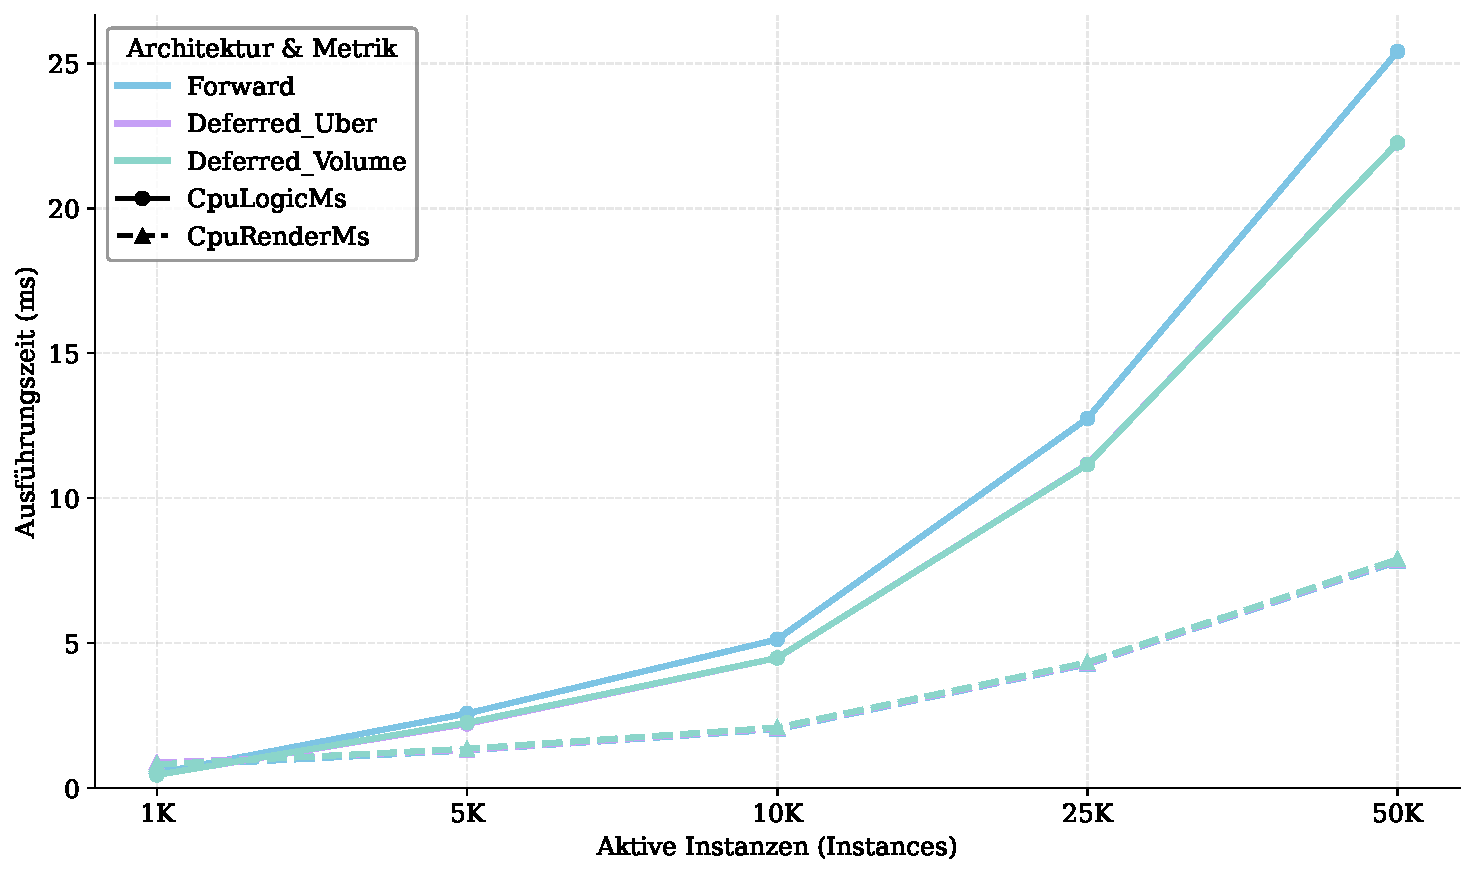
\includegraphics[width=0.9\linewidth]{Abbildungen/5_2_2_cpu_scaling_logic_vs_render}
    \caption[Objektanzahl-Limitierung im CPU-Dispatch]{Messung von \texttt{CpuLogicMs} und \texttt{CpuRenderMs} bei
    einer Skalierung von 1.000 bis 50.000 Instanzen zur Isolation der CPU-Architektur.}
    \label{fig:5_2_2_cpu_scaling_logic_vs_render}
\end{figure}

\subsection{{Overdraw-Dichte}}
\label{subsec:050203_overdraw_eval}

\begin{figure}[htbp]
    \centering
    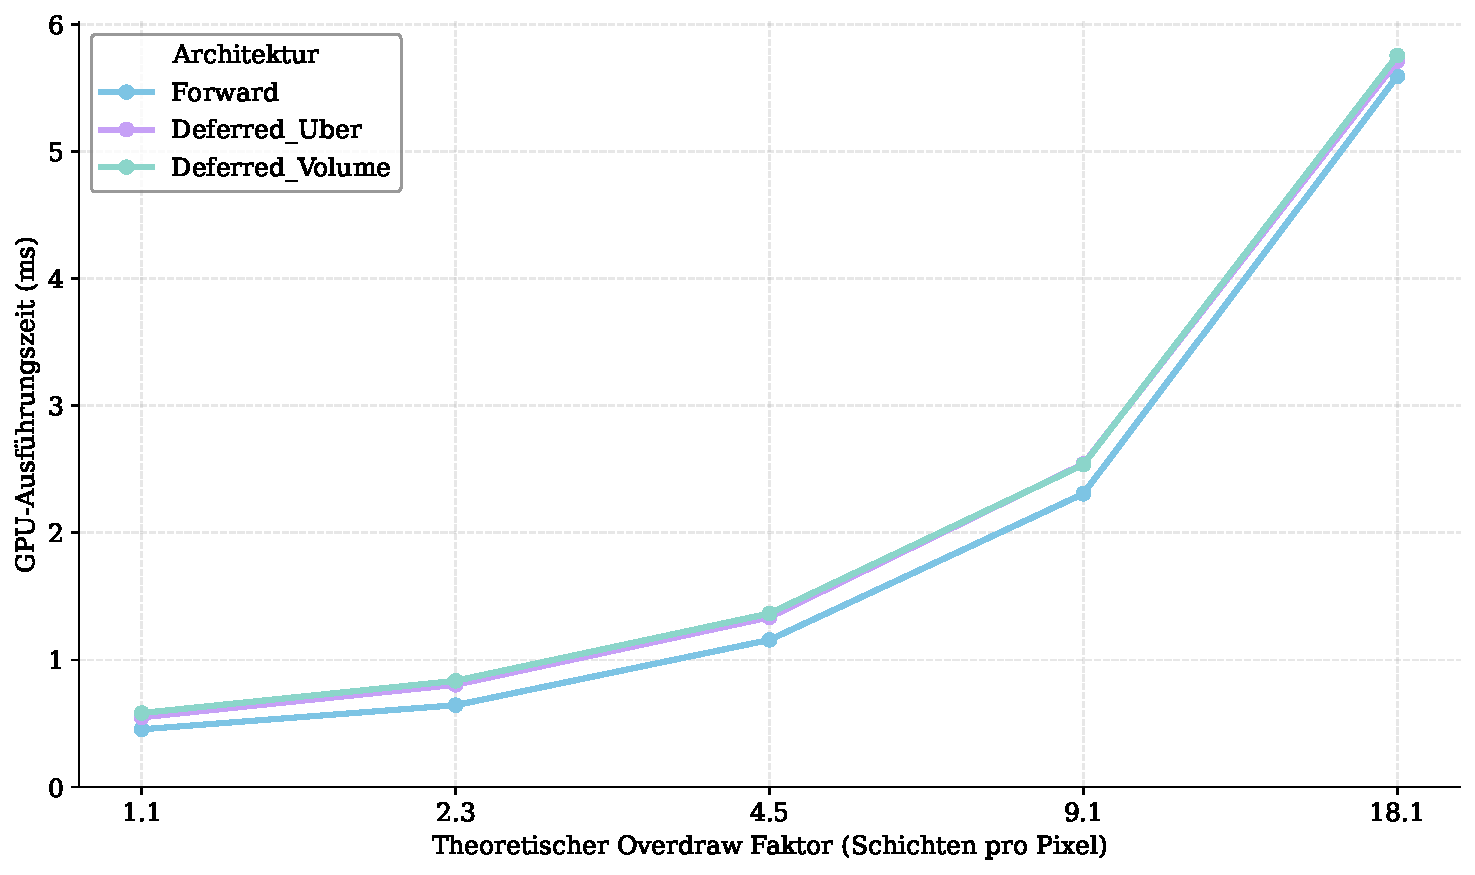
\includegraphics[width=0.9\linewidth]{Abbildungen/5_2_3_overdraw_fillrate_scaling}
    \caption[Overdraw-Skalierung bei steigender Tiefenkomplexität]{Messung der GPU-Ausführungszeit in Abhängigkeit vom
    theoretischen Overdraw-Faktor (1,1 bis 18,1 Schichten pro Pixel) bei einer Skalierung von 2.000 bis 32.000
    Instanzen.}
    \label{fig:5_2_3_overdraw_fillrate_scaling}
\end{figure}


\section{{Bandbreite und Auflösung}}
\label{sec:0503_brandwidth_resolution_eval}

In dem nachfolgenden Kapitel werden Benchmarks und Erkenntnisse präsentiert, die dazu dienen, die
bandbreitenspezifischen Limitierungen auszuloten.
Im Rahmen der Analyse werden die API und die Speicherkosten des G-Buffers sowie der zunehmende ALU-Aufwand des
Forward-Rendering evaluiert.

\subsection{{Auflösung}}
\label{subsec:050301_resolution_eval}

\begin{figure}[htbp]
    \centering
    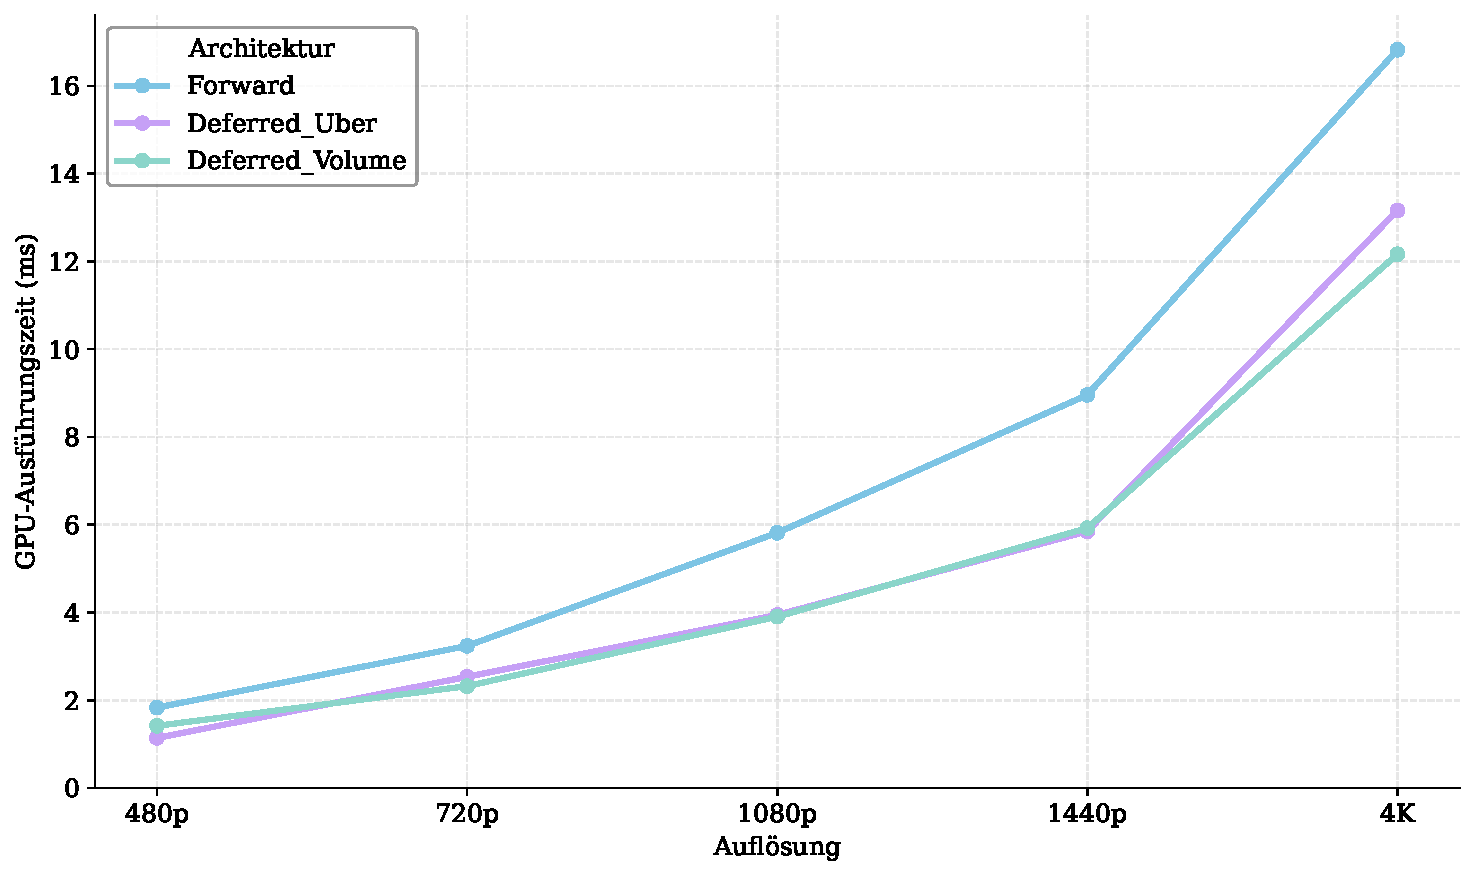
\includegraphics[width=0.9\linewidth]{Abbildungen/5_3_1_resolution_scaling_crossover}
    \caption[Auflösungsskalierung unter konstanter Beleuchtungslast]{Messung der GPU-Ausführungszeit in Abhängigkeit von
    der Framebuffer-Auflösung (480p bis 4K) unter einer statischen Last von 100 Lichtquellen.}
    \label{fig:5_3_1_resolution_scaling_crossover}
\end{figure}

\subsection{{Bandbreiten}}
\label{subsec:050302_bandwidth_eval}

\begin{figure}[htbp]
    \centering
    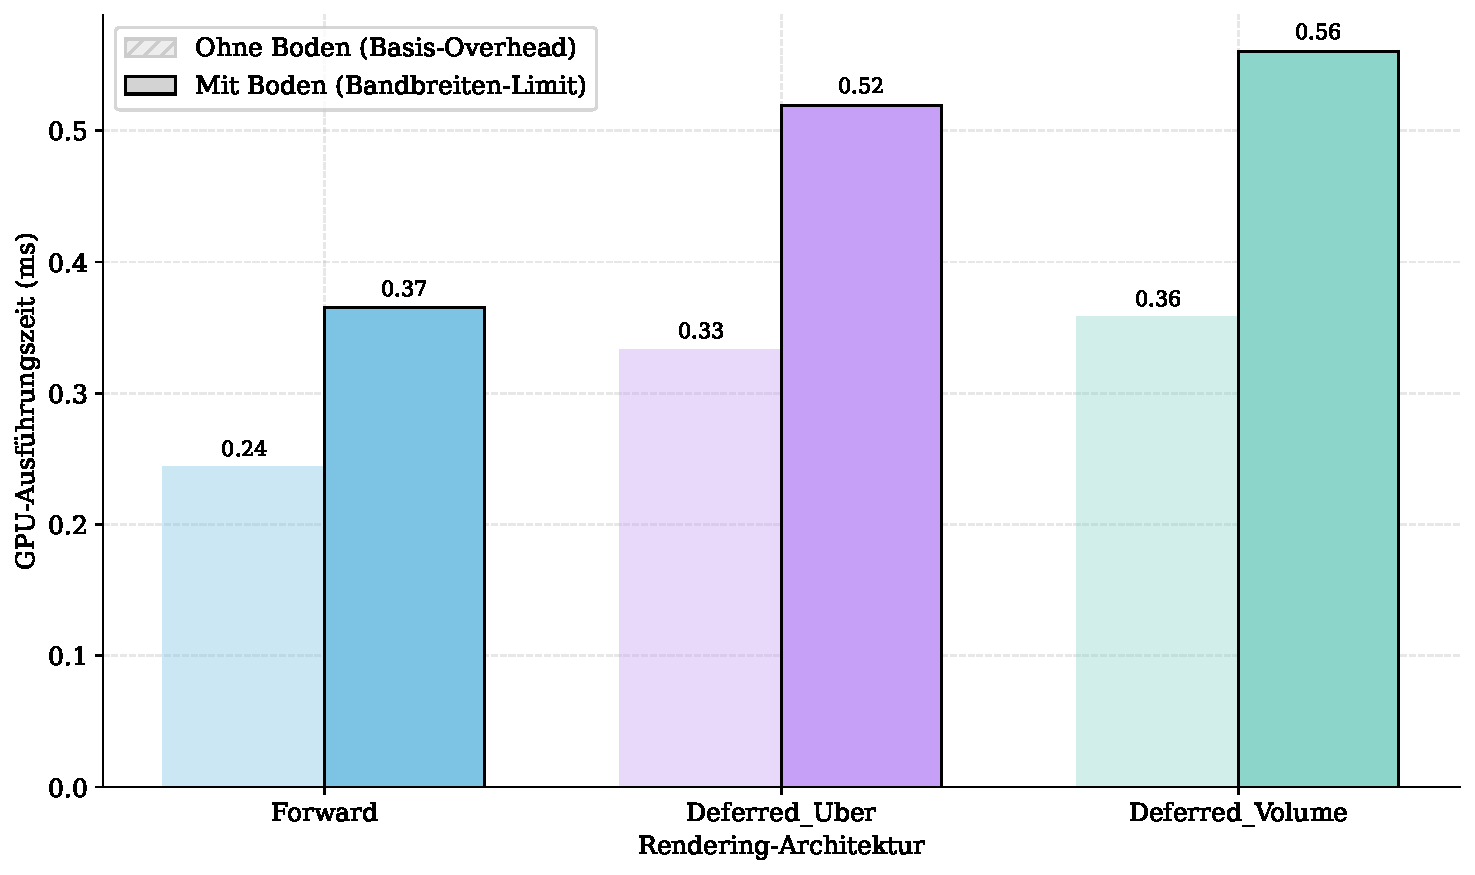
\includegraphics[width=0.9\linewidth]{Abbildungen/5-3-2_BaseBandwidthTax_Means}
    \caption[Basis-Bandbreitenkosten der Rendering-Architekturen]{Vergleich der GPU-Ausführungszeit zwischen minimaler
    Geometrielast (Basis-Overhead) und vollflächiger Screen-Space-Abdeckung (Bandbreiten-Limit) ohne Beleuchtung zur
    Isolierung der G-Buffer-Speicherbandbreite.}
    \label{fig:5_3_2_base_bandwidth_tax_means}
\end{figure}


\section{{Beleuchtung}}
\label{sec:0504_lighting_eval}

Im nachfolgenden Kapitel werden Benchmarks und Erkenntnisse präsentiert, die dazu dienen, die beleuchtungsspezifischen
Limitierungen zu ermitteln.
Da Deferred Rendering im Bereich der Beleuchtungsberechnung signifikante Vorteile verspricht, sollen im Folgenden die
genauen architektonischen Crossover-Points ermittelt werden, ab denen die Deferred-Pipelines die Forward-Pipelines
übertreffen.
Auf Hardware-Ebene werden im Rahmen der vorliegenden Untersuchung die ALU- und ROP-Limits mithilfe der nachfolgenden
Benchmarks evaluiert.

\subsection{{Lichtanzahl}}
\label{subsec:050401_light count_eval}

\begin{figure}[htbp]
    \centering
    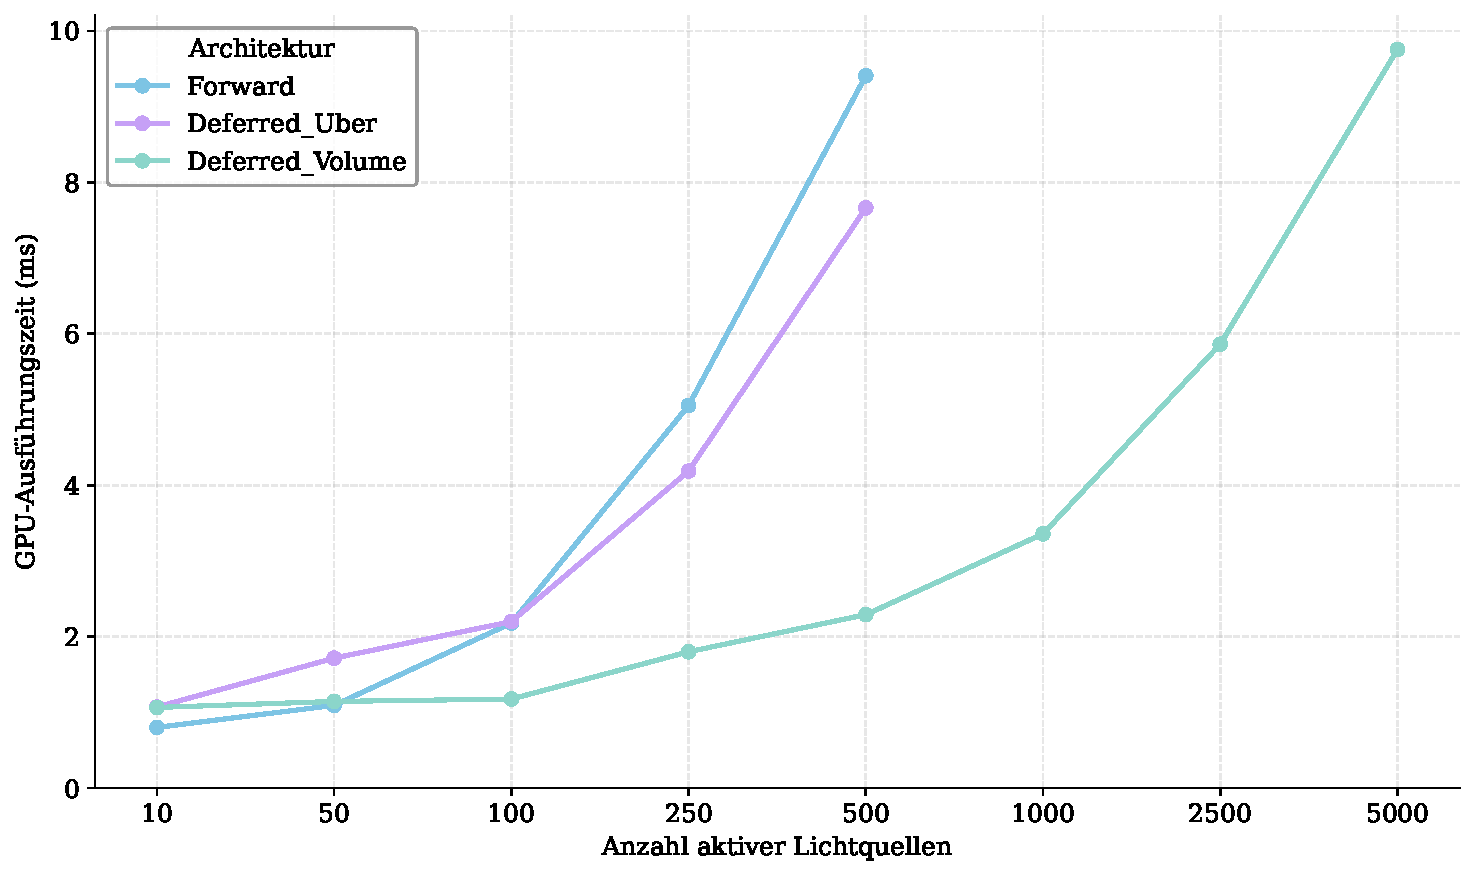
\includegraphics[width=0.9\linewidth]{Abbildungen/5-4-1_LightCount_Means}
    \caption[Skalierung der Lichtanzahl bei dynamischen Punktlichtern]{Messung der GPU-Ausführungszeit in Abhängigkeit
    von der Anzahl aktiver Lichtquellen (10 bis 5.000).}
    \label{fig:5_4_1_light_count_means}
\end{figure}

\subsection{{Lichtintensität \& Overlap}}
\label{subsec:050402_light_intensity_and_overlap_eval}

\begin{figure}[htbp]
    \centering
    
\includegraphics[width=0.9\linewidth]{Abbildungen/5-4-2-1_LightIntensity_Means}
    \caption[Skalierung der Lichtintensität bei konstanter Lichtanzahl]{Messung der GPU-Ausführungszeit in Abhängigkeit
    von der Lichtintensität respektive dem Radius-Multiplikator (0,5 bis 20,0) bei einer konstanten Anzahl von 250
    Lichtquellen.}
    \label{fig:5_4_2_1_light_intensity_means}
\end{figure}

\begin{figure}[htbp]
    \centering
    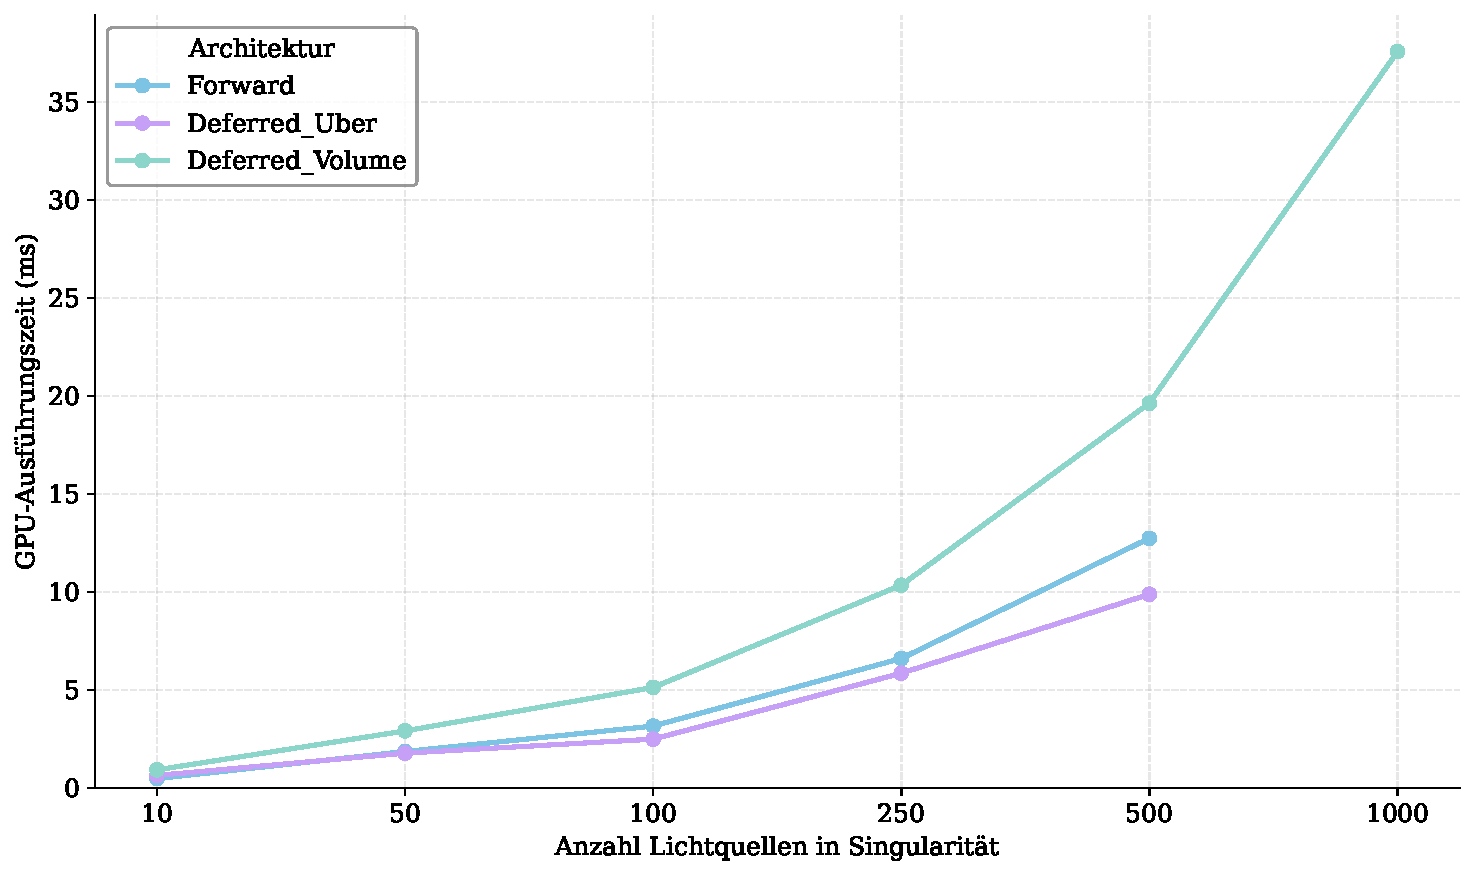
\includegraphics[width=0.9\linewidth]{Abbildungen/5-4-2-2_LightSingularity_Means}
    \caption[Skalierung der Lichtanzahl in einer Singularität]{Messung der GPU-Ausführungszeit in Abhängigkeit von der
    Anzahl der Lichtquellen (10 bis 1000) bei einer Positionierung aller Lichtquellen in einer räumlichen Singularität.}
    \label{fig:5_4_2_2_light_singularity_means}
\end{figure}

\subsection{{Shading Overdraw}}
\label{subsec:050403_shading_overdraw_eval}

\begin{figure}[htbp]
    \centering
    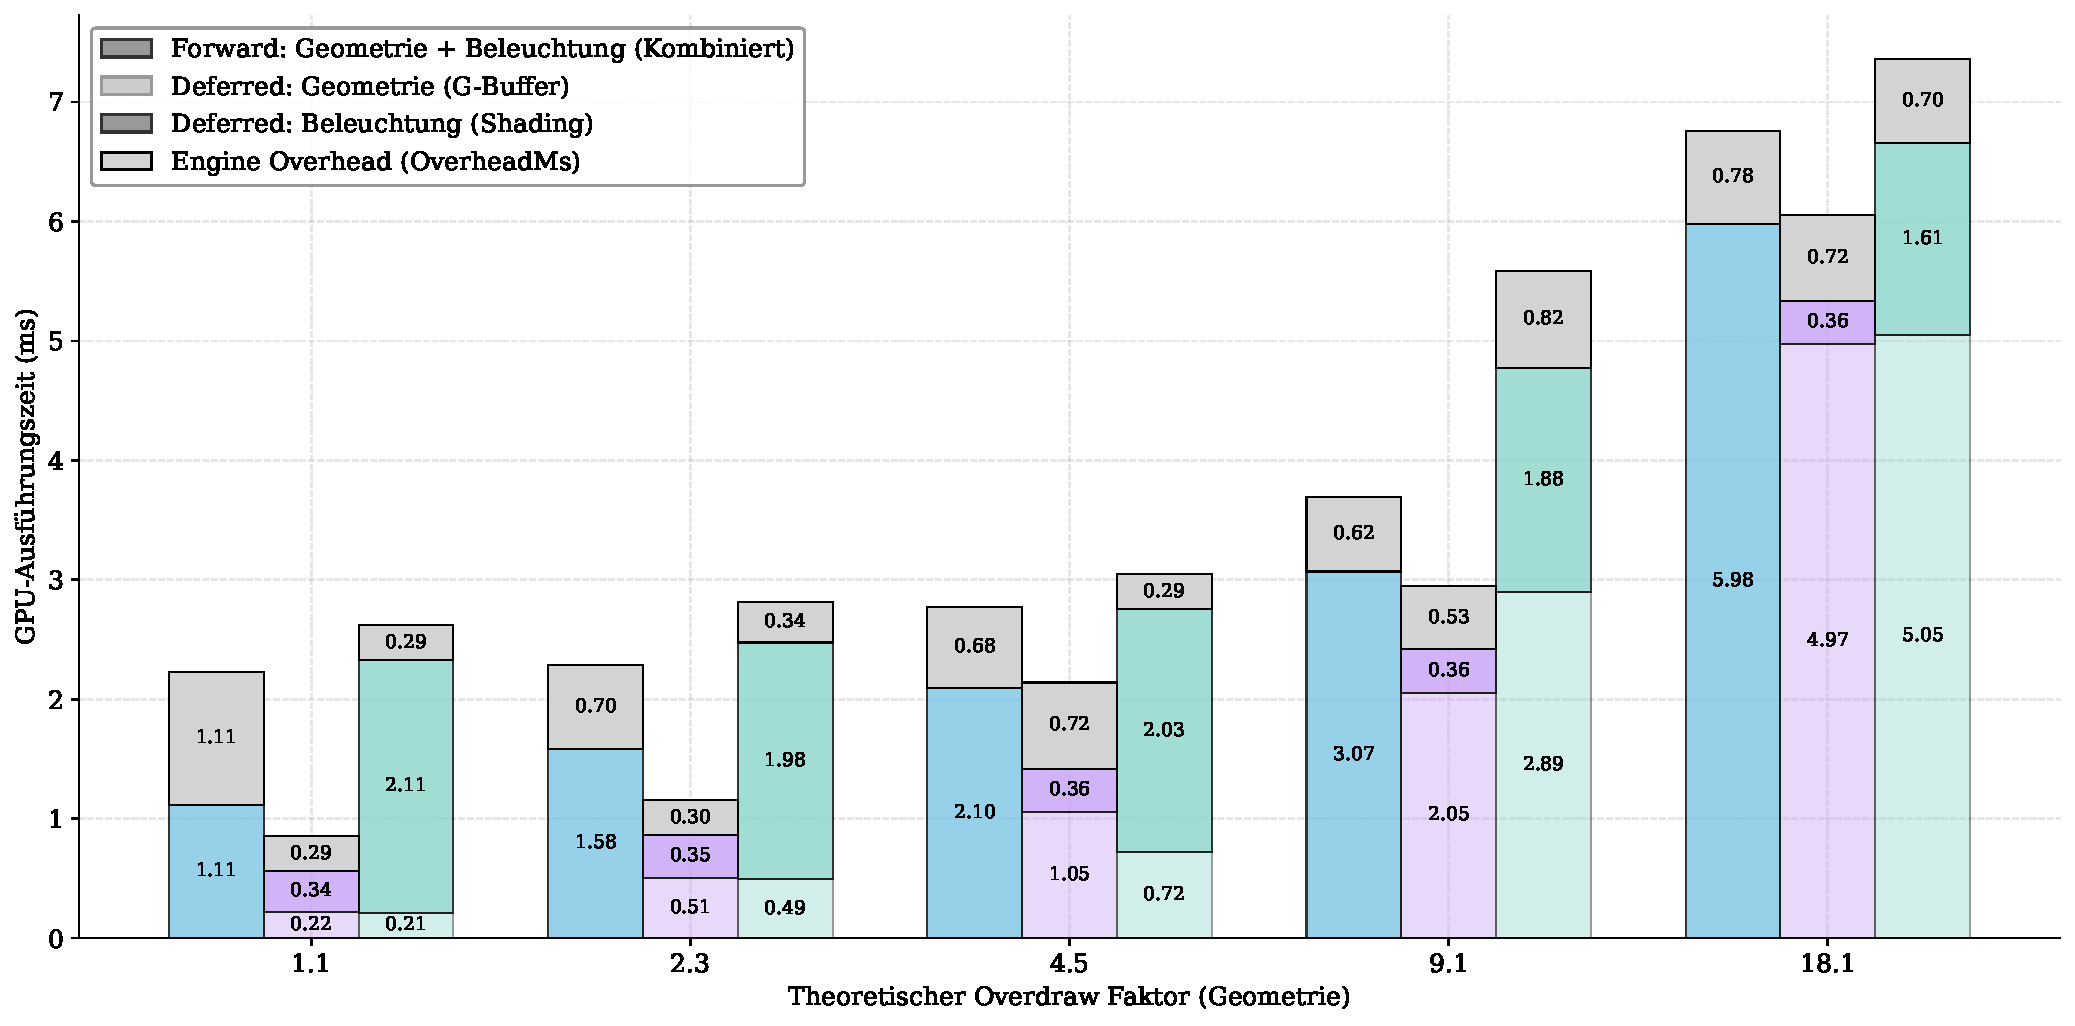
\includegraphics[width=0.9\linewidth]{Abbildungen/5_4_3_decoupling_proof}
    \caption[Entkopplungsnachweis bei steigendem geometrischen Overdraw]{Aufschlüsselung der GPU-Ausführungszeit nach
    einzelnen Pipeline-Komponenten in Abhängigkeit vom theoretischen Overdraw-Faktor bei einer konstanten Last von 100
    Lichtquellen.}
    \label{fig:5_4_3_decoupling_proof}
\end{figure}


\section{{Hybride Stilisierung \& Entropie}}
\label{sec:0505_npr_eval}

In den vorangegangenen Kapiteln 5.2 bis 5.4 wurde das grundlegende Verhalten der evaluierten Rendering-Architekturen
aufgezeigt und somit zugleich die Fähigkeiten und Grenzen des HyDra-Frameworks als Kontrollgruppen demonstriert.
Die nachfolgenden Tests widmen sich dem Kern der Forschung und evaluieren die Wechselwirkungen von Stil-Entropie und
den allgemeinen Einfluss selektiver NPR-Techniken auf die verschiedenen Pipelines.
Der Fokus liegt hierbei insbesondere auf der Evaluation von Warp Divergence und Register Pressure.

\subsection{{Stil-Entropie}}
\label{subsec:050501_entropy_eval}

\begin{figure}[htbp]
    \centering
    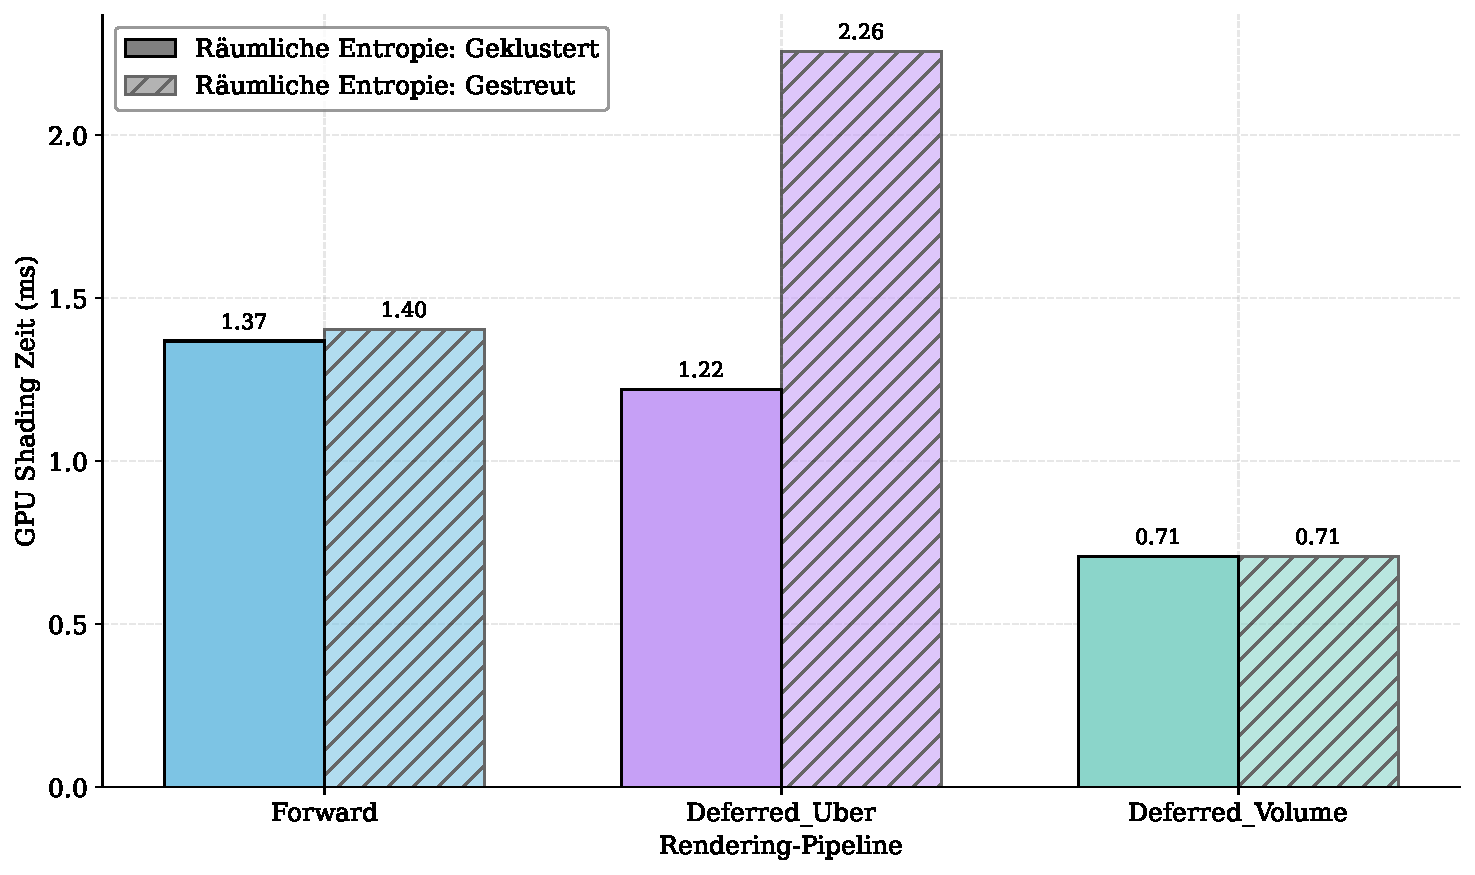
\includegraphics[width=0.9\linewidth]{Abbildungen/5_5_1_entropy_divergence_means}
    \caption[Einfluss der räumlichen Entropie auf die GPU-Shading-Zeit]{Messung der GPU-Shading-Zeit in Abhängigkeit von
    der räumlichen Verteilung (Geklustert vs. Gestreut) der Rendering-Stile zur Isolation von Warp Divergence.}
    \label{fig:5_5_1_entropy_divergence_means}
\end{figure}

\begin{figure}[htbp]
    \centering
    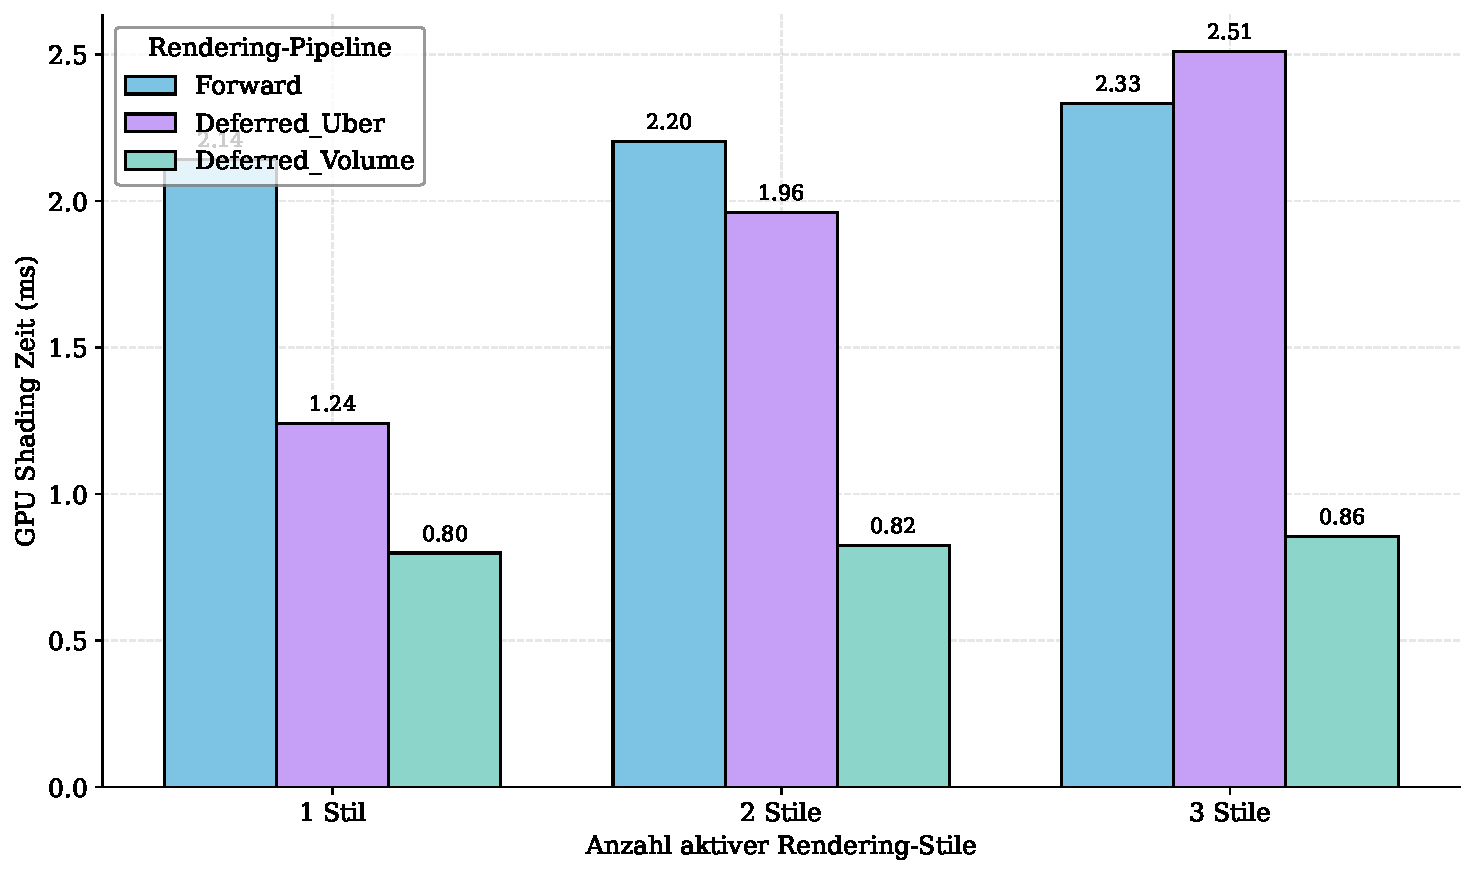
\includegraphics[width=0.9\linewidth]{Abbildungen/5_5_2_style_combinatorics_gpu}
    \caption[Einfluss stilistischer Kombinatorik auf die GPU-Shading-Zeit]{Messung der GPU-Shading-Zeit in Abhängigkeit
    von der Anzahl simultan aktiver Rendering-Stile (1 bis 3 Stile) zur Evaluierung kombinatorischer Degradation.}
    \label{fig:5_5_2_style_combinatorics_gpu}
\end{figure}

\subsection{{Kernel Bandbreiten Limits}}
\label{subsec:050502_kernel_eval}

\begin{figure}[htbp]
    \centering
    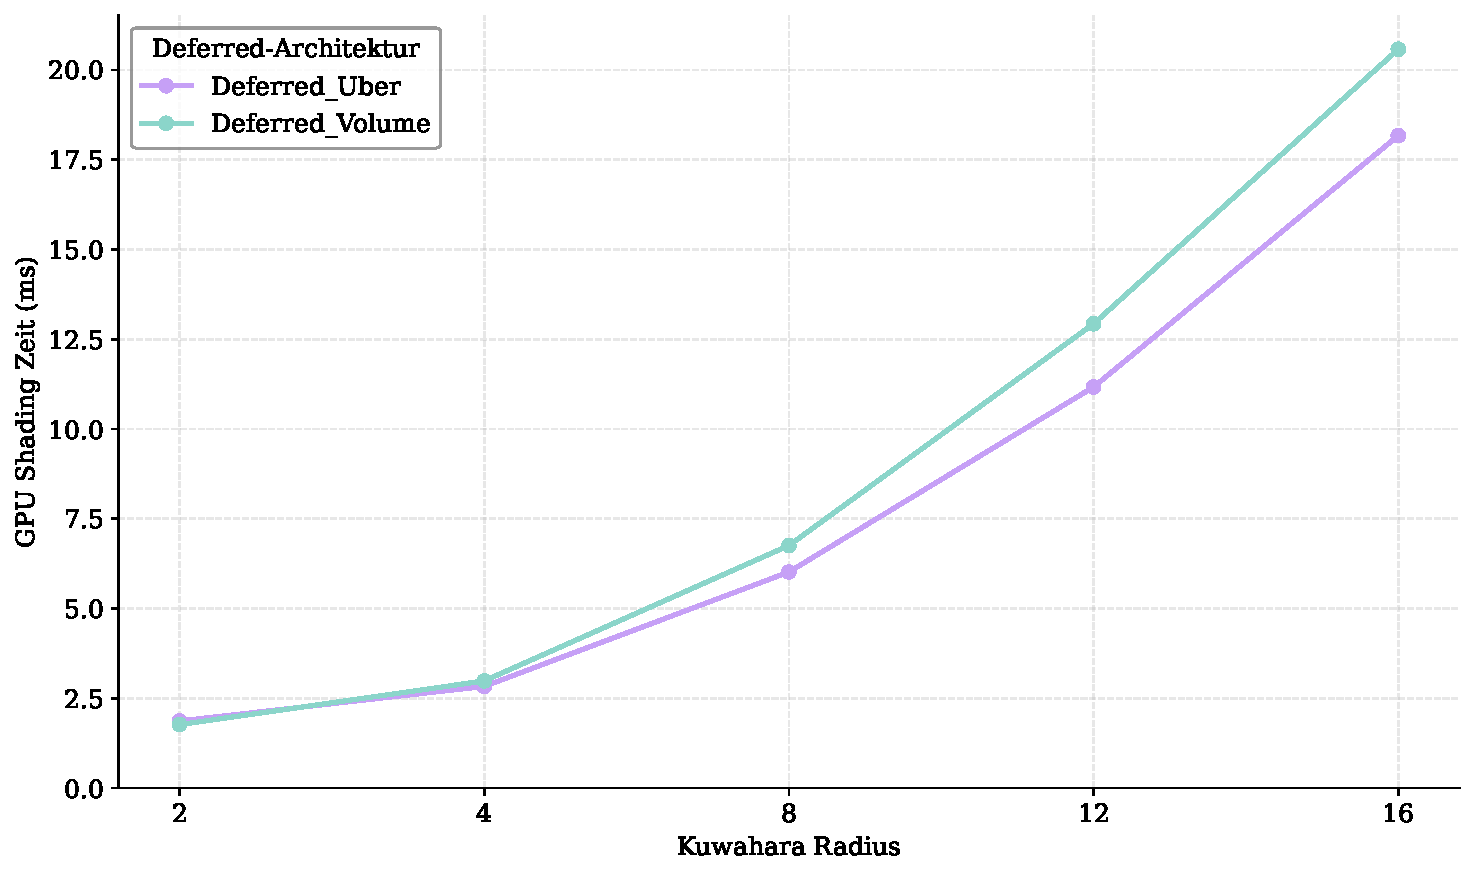
\includegraphics[width=0.9\linewidth]{Abbildungen/5_5_3_kernel_bandwidth_scalability}
    \caption[Skalierung des Kuwahara-Filterradius]{Messung der GPU-Shading-Zeit in Abhängigkeit vom
    Kuwahara-Kernel-Radius (2 bis 16) zur Evaluation der VRAM-Bandbreitenlimits unter steigender Filtergröße.}
    \label{fig:5_5_3_kernel_bandwidth_scalability}
\end{figure}


\section{{Macro-Benchmark Synthese}}
\label{sec:0506_kernel_eval}

In der finalen Testreihe erfolgt die Integration aller übergeordneter Einflüsse aus den vorangegangenen Benchmarks in
ein umfassendes Real-World-Szenario, um die Interaktion der bislang untersuchten Effekte in ihrer Gesamtheit zu
analysieren.
Die nachfolgenden Evaluationen werden in einem Schritt zusammengefasst, bestehen allerdings aus vier verschiedenen
Einzelpässen, in welchen die verschiedenen Einflüsse von Geometrie, Beleuchtung und selektiver Silisierung gemeinsam
betrachtet werden.

\begin{figure}[htbp]
    \centering
    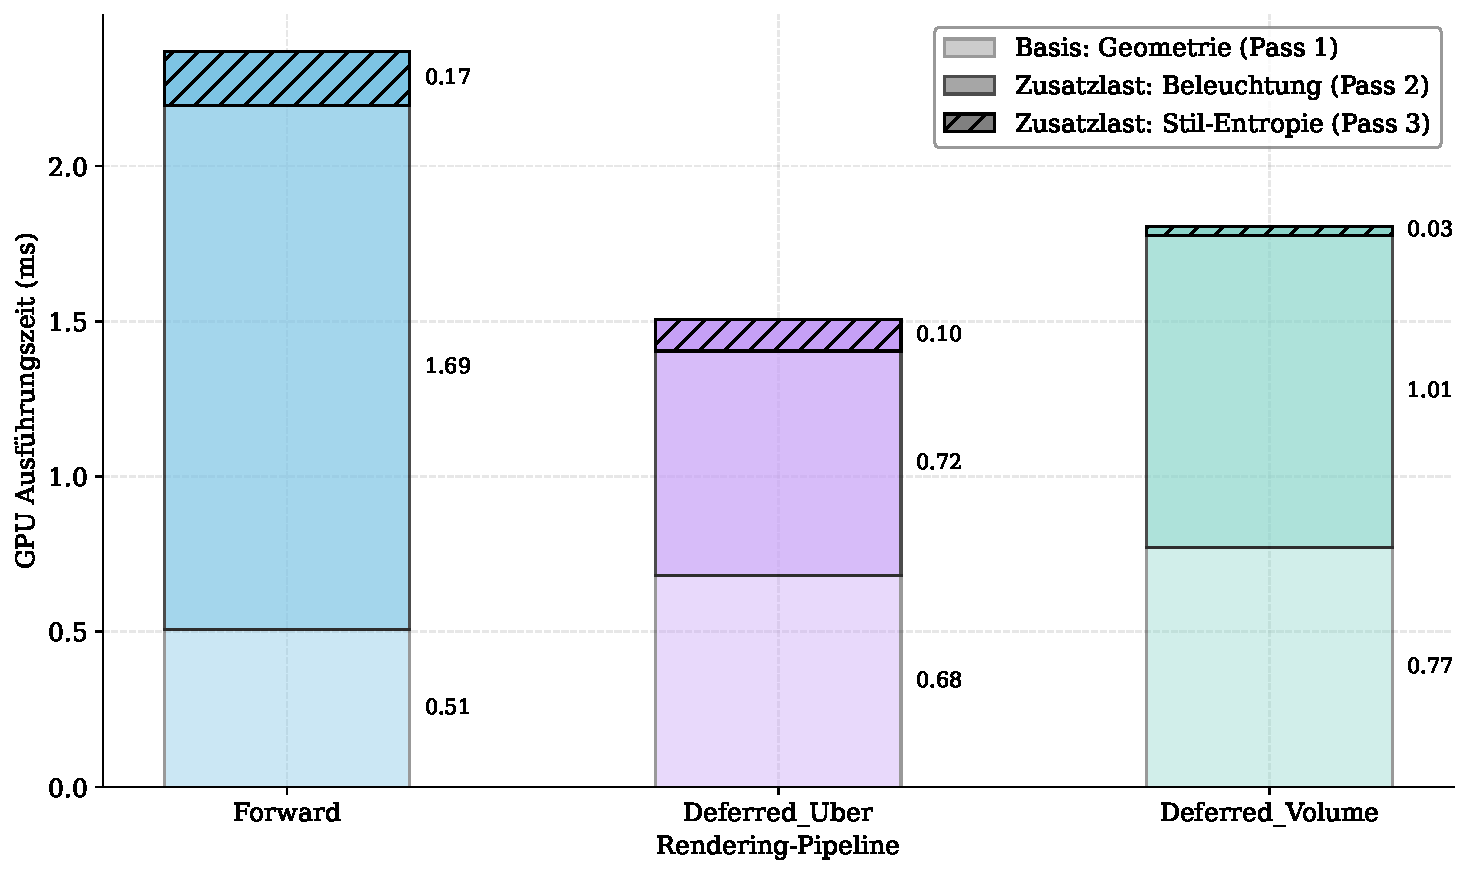
\includegraphics[width=0.9\linewidth]{Abbildungen/5_6_cumulative_rendering_cost_combined}
    \caption[Akkumulierte GPU-Ausführungszeit im Makro-Benchmark]{Aufschlüsselung der GPU-Ausführungszeit nach
    Pipeline-Komponenten (Geometrie, Beleuchtung und Stil-Entropie).}
    \label{fig:5_6_cumulative_rendering_cost_combined}
\end{figure}

\begin{figure}[htbp]
    \centering
    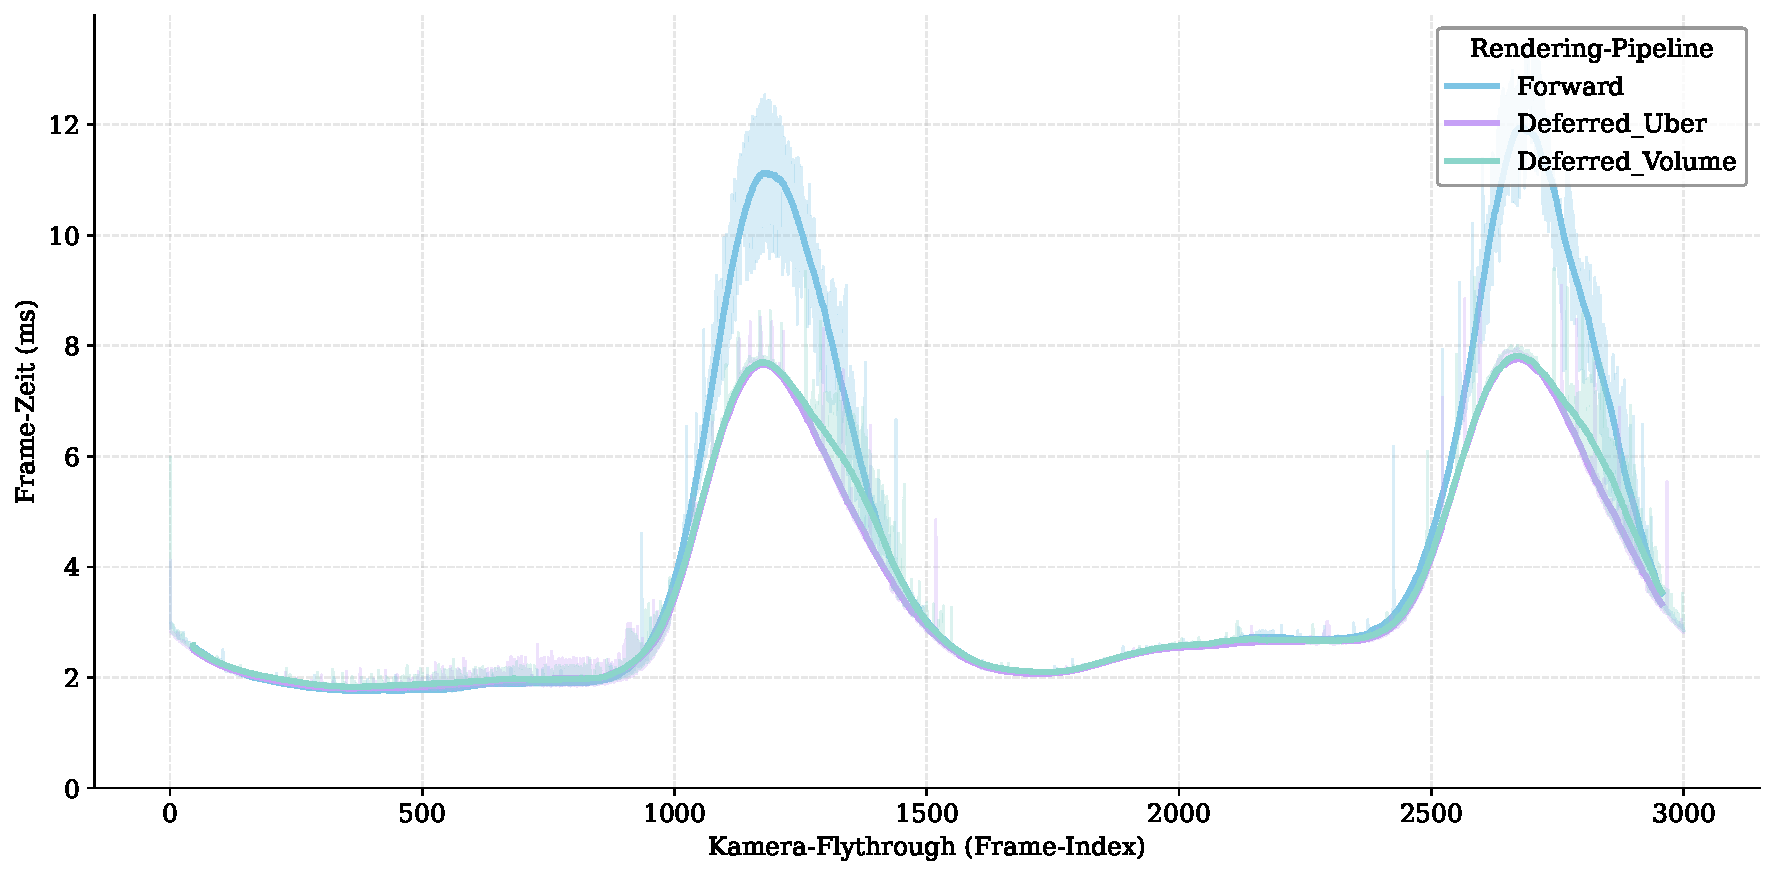
\includegraphics[width=0.9\linewidth]{Abbildungen/5_6_flythrough_variance}
    \caption[Frame-Zeit-Verlauf des Kamera-Flythroughs]{Verlauf der Frame-Zeit über die Dauer von 3000 Frames des
    Kamera-Flythroughs unter kombinierter Geometrie-, Beleuchtungs- und Stil-Last.}
    \label{fig:5_6_flythrough_variance}
\end{figure}
